\documentclass{standalone}
\usepackage{tikz}
\usetikzlibrary{shapes.geometric, arrows, positioning}

\begin{document} 
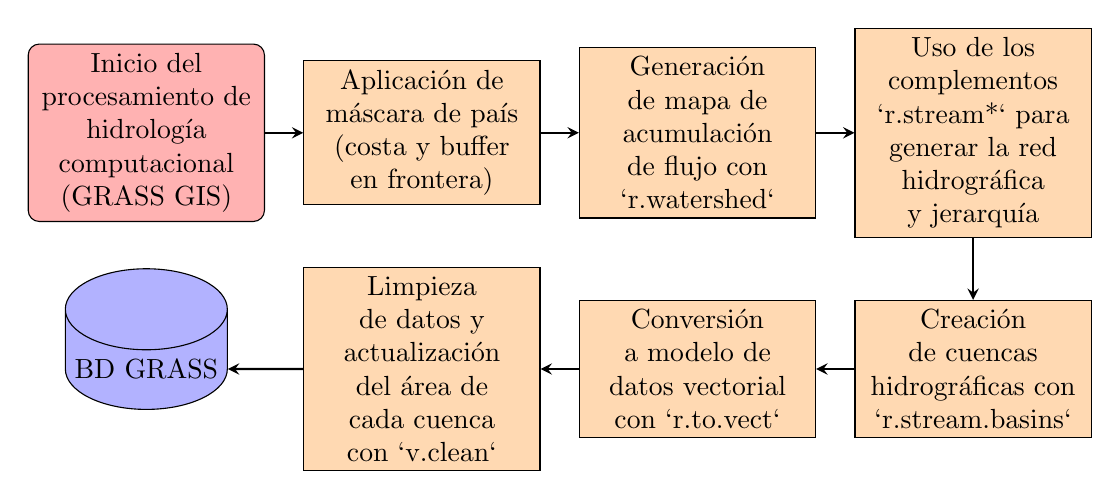
\begin{tikzpicture}[
  startstop/.style={rectangle, rounded corners, minimum width=3cm, minimum height=1cm,text centered, align=center, draw=black, fill=red!30},
  db/.style={cylinder, shape border rotate=90, aspect=0.5, draw, fill=blue!30},
  io/.style={trapezium, trapezium left angle=70, trapezium right angle=110, minimum width=3cm, minimum height=1cm, text centered, align=center, draw=black, fill=blue!30},
  process/.style={rectangle, minimum width=3cm, minimum height=1cm, text centered, align=center, draw=black, fill=orange!30},
  decision/.style={diamond, minimum width=3cm, minimum height=1cm, text centered, align=center, draw=black, fill=green!30},
  arrow/.style={thick,->,>=stealth}]

  % Nodes
  \node (start) [startstop] {Inicio del \\ procesamiento de \\ hidrología \\ computacional \\ (GRASS GIS)};
  \node (mask) [process, right of=start, xshift=2.5cm] {Aplicación de \\ máscara de país \\ (costa y buffer \\ en frontera)};
  \node (rwatershed) [process, right of=mask, xshift=2.5cm] {Generación \\ de mapa de \\ acumulación \\ de flujo con \\ `r.watershed`};
  \node (rstream) [process, right of=rwatershed, xshift=2.5cm] {Uso de los \\ complementos \\ `r.stream*` para \\ generar la red \\ hidrográfica \\ y jerarquía};
  
  \node (rbasins) [process, below of=rstream, yshift=-2cm] {Creación \\ de cuencas \\ hidrográficas con \\ `r.stream.basins`};
  \node (rtovect) [process, left of=rbasins, xshift=-2.5cm] {Conversión \\ a modelo de \\ datos vectorial \\ con `r.to.vect`};
  \node (vclean) [process, left of=rtovect, xshift=-2.5cm] {Limpieza \\ de datos y \\ actualización \\ del área de \\ cada cuenca \\ con `v.clean`};
  \node (end) [db, left of=vclean, xshift=-2.5cm] {BD GRASS};

  % Arrows
  \draw [arrow] (start) -- (mask);
  \draw [arrow] (mask) -- (rwatershed);
  \draw [arrow] (rwatershed) -- (rstream);
  
  \draw [arrow] (rstream) -- (rbasins);
  \draw [arrow] (rbasins) -- (rtovect);
  \draw [arrow] (rtovect) -- (vclean);
  \draw [arrow] (vclean) -- (end);
\end{tikzpicture}
\end{document}
